%%=============================================================================
%% testen van de Automated reconnaissance tools
%%=============================================================================
% \chapter{Automated reconnaissance tools}
% \label{ch:Automated reconnaissance tools}

\chapter{\IfLanguageName{dutch}{Tool evaluatie}{Tool evaluatie}}
\label{ch:geautomatiseerde Reconnaissance}

\section{Methodology voor tool evaluatie}

De reconnaissancefase werdt uitgevoerd in een gecontroleerde virtuele omgeving (zie~\ref{ch:Proof of Concept} Proof of Concept) om de manuele en geautomatiseerde tools te evalueren.
Deze evaluatie is uitgevoerd met het OSSTMM framework, met nadruk op het standaardiseren, de reproduceerbaarheid, de secties en neutraliteit.
De manuele reconnaissance is uitgevoerd gebruik makende van 54 commando's. 
Deze zijn gekozen om een zo breed mogelijke oppervlakte te dekken van de reconnaissancefase, verdeeld over vijf categorieën.
De geautomatiseerde reconnaissance is uitgevoerd gebruik makende van zeven verschillende tools: AutoRecon, CyberScan, LazyRecon, Sn1per, RustScan, Nuclei en ReconFTW.
Dit hoofdstuk zal een gedetailleerde vergelijking maken, kijkende naar de betrouwbaarheid, uitvoeringstijd, bruikbaarheid, het CPU-gebruik en de OSSTMM RAV-score.

% deze comanandos zijn uitgevoer in een gecontroleerde omgeving zie hoofdstuk ref{ch:PoC}, deze bieden ook een baselinen voor de evaluatie voor de geautomatiseerde tools.
% De manuele reconnaisansse is een belangerijk deel van deze bachelorproef.
% De manuele reconnaisanse is uitgevoerd voor de effectiviteiet van de individuele tools te testen binnen de OSSTMM framwork.
% Deze aanpak heb ik ondernomen door een zo breed moeglijke scala aan tools te gebruiken en met de informatie die er daar verzamleld werdt verder onderzocht im al de mogelijke kwetsbaarheden opn te leggen.
% Uit de manuele test is er een bash script opgesteld om de betroubaarheid van de tool, tijd en cpu gebruik te testen.
% In dit hooofdstuk zal de manuele reconnaisanse proces overlopen worden, categorisatie van 54 comanandos in 5 OSSTMM categorieen, de automatisatie van de 

\section{Manuele reconnaissance}
De manuele reconnaissance werd uitgevoerd op Kali Linux 2024.2 (\texttt{192.168.56.10}) met doelwit Metasploitable2 (\texttt{192.168.56.11}) over een geïsoleerd virtueel netwerk (zie~\ref{ch:Proof of Concept} Proof of Concept).
Het uitvoeren van de manuele reconnaissance gebruikte 54 commando's, ieder commando is uitgekozen om elk aspect van de reconnaissance te dekken, wat gedefinieerd was in het OSSTMM Data network en Human secties (zie tabel~\ref{tab:recon} Reconnaissance activiteiten gemaped naar OSSTMM secties en RAV metrics).
De commando's zijn manueel getest om de output, uitvoertijd en mogelijke foutmeldingen te verstaan, ze zijn opgeslagen in een tabel (zie~\ref{tab:vergelijking-recon-manueel} Vergelijking van manuele reconnaissance-tools).
Na het uitvoeren van al de commando's is er een bash script opgezet om de betrouwbaarheid van te tool, de uitvoeringstijd en het CPU-gebruik te testen.

\subsection{Categorisatie van de commando's}

Om een structuur in reconnaissance te brengen zijn de 54 commando's georganiseerd in vijf categorieën, gebaseerd op hun functionaliteit en overeenkomst met de OSSTMM objectieven (Standaardiseren, Reproduceerbaar, Neutraal, Meetbare risico).
De categorieën zijn als volgt:

\begin{itemize}
  \item \textbf{netwerk en host discovery} geeft de actieve hosts en Netwerk configuraties;
    {\scriptsize \begin{itemize}
      \item \textmd{RAV-score} V: hoog, A: laag, T: laag
    \end{itemize} }
  \item \textbf{poorten en service analyse} scans voor open poorten en lopende services;
    {\scriptsize \begin{itemize}
      \item \textmd{RAV-score} V: hoog, A: Medium, T: Low
    \end{itemize} }
  \item \textbf{web reconnaissance} webservers en toepassingen weergeven;
    {\scriptsize \begin{itemize}
      \item \textmd{RAV-score} V: hoog, A: Medium, T: Medium
    \end{itemize} }
  \item \textbf{protocol en service enumeratie } geeft specifieke protocollen en services weer;
  {\scriptsize \begin{itemize}
    \item \textmd{RAV-score} V: Medium, A: hoog, T: hoog
  \end{itemize} }
  \item \textbf{vulnerability scanning} detecteert mogelijke exploits en kwetsbaarheden.
  {\scriptsize \begin{itemize}
    \item \textmd{RAV-score} V: hoog, A: hoog, T: Medium
  \end{itemize} }
\end{itemize}
  
\subsection{Manuele uitvoer}
Deze commando's zijn manueel uitgevoerd, waar voor de output van de commando's opgeslagen zijn in een tabel (zie~\ref{tab:vergelijking-recon-manueel} Vergelijking van manuele reconnaissance-tools).
De observaties zijn als volgt:

\begin{itemize}
  \item \textbf{uitvoeringstijd:} de uitvoer van de commando's varieert extreem van 0.01 seconde naar 521 seconden;
  \item \textbf{betrouwbaarheid:} sommige commando's falen door Metasploitable2 onstabiele services, wat voor betrouwbaarheidsprobemen kan zorgen.
  \item \textbf{bruikbaarheid:} interactieve commando's vragen manuele input, wat de uitvoer tijd en complexiteit moeilijker maken. Het gebruik en interpretatie van de tool hangt af van de ervaring en kennis van de pentester.
  \item \textbf{RAV-score:} de RAV-score is zeer variabel, dit geeft de betrouwbaarheid en de bruikbaarheid van de tool aan.

\end{itemize}

Deze manuele reconnaissance geeft diepe inzichten in de werking van de Metasploitable2 en de verschillende services die erop staan.
Echter is dit tijdrovend, repetetief, error gevoelig en staan het merendeel van de commando's niet in deze vergelijking aangezien deze niet bruikbaar zijn voor deze specifieke case.

\subsection{Bash script voor betrouwbaarheid}

Om de betrouwbaarheid te kunnen testen is er een bash script opgezet dat de 54 commando's bevat (zie~\ref{lst:recon-script} Reconnaissance bash Script). Het script is gemaakt om de betrouwbaarheid door consistentie te testen maar ook de error en time-out frequentie te bepalen.
Dit script bevat:

\begin{itemize}
  \item \textbf{commando's organisatie} de commando's zijn georganiseerd in vijf verschillende categorieën, deze zijn opgeslagen in een matrix voor een modulaire uitvoering;
  \item \textbf{3x testen} de commando's zijn drie maal uitgevoerd om de consistentie, tijd stabiliteit, error en time-out frequentie, en het CPU-gebruik te testen;
  \item \textbf{output structuur} de resultaten zijn opgeslagen in zijn categorie specifieke tekstbestand, hierin zit de commando output, tijd, het CPU-gebruik, de error en time-out status;
  \item \textbf{interactieve commando's} de interactieve commando's werden vervangen door alternatieve, niet-interactieve commando's, zo wordt de automatisatie van het script vervolledigd. 
  \item \textbf{error handling} de errors en time-outs worden opgevangen en gelogd in een aparte tekst bestand.

\end{itemize}

\subsection{Bash script uitvoer}

Deze uitvoer van het bash script is ingedeeld in vijf categorieën: vulnerability scanning, protocol en service enumeratie, poort en service analyse, netwerk en host ontdekking, Web Reconnaissance.
De meeste commanando's waren consistent over de drie runs, met enkele uitzonderingen waar er inconsistentie en fouten optraden.
Dat wijst op een betrouwbare uitvoering binnen de virtuele omgeving.

De uitvoering van het bash script leverde de volgende resultaten:

\begin{itemize}
  \item \textbf{consistentie} de meeste commandos uit het bash script zijn consistent over de drie runs, met enkele uitzonderingen waar er inconsistentie en fouten optraden;
  \item \textbf{foutfrequentie} tien procent van alle commando's gaf een foutmelding of time-out. De meeste fouten kwamen voor bij de \textit{vulnerability-scanning} en \textit{protocol- en service-enumeratie} categorieën;
  \item \textbf{RAV-score impact} de output consistentie bepaalt de RAV-scores, een stabiele output verhoogt de \textit{visibility}- en \textit{access} scores.
  
\end{itemize}


De uitvoeringstijden en het CPU-verbruik werden ook berekend per categorie, door de totale tijd en het CPU-gebruik te nemen van alle commando's per categorie per run op te sommen uit te delen over de drie runs.

% 
% De uitvoeringstijden varieerden per categorie, met poort analyse en netwerk discovery als snelste (~7-37sec) en vulnerability scanning als meest tijdrovende (~37sec).
% De CPU verbruik schommeld veel van 0\% tot 104\% dit komt door dat de metingen gebreuren op de totale gebruik van alle cpu cores. waar de gemiddelde geberuik bij de categorie web reconnaissance het hoogst was (~46\%).


\begin{table}[h]
  \centering
  \footnotesize
  \begin{tabular}{lcc}
  \toprule
  \textbf{Categorie} & \textbf{Gemiddelde Uitvoeringstijd (per run)} & \textbf{Gemiddeld CPU-Gebruik} \\
  \midrule
  Vulnerability Scanning & $\sim$51 seconden & 17\% \\
  Protocol en Service Enumeratie & $\sim$5 seconden & 24\% \\
  Poort en Service Analyse & $\sim$33 seconden & 9\% \\
  Netwerk en Hostontdekking & $\sim$7 seconden & 36\% \\
  Web Reconnaissance & $\sim$6 seconden & 46\% \\
  \bottomrule
  \end{tabular}
  \caption{Gemiddelde uitvoeringstijd en CPU-gebruik per categorie}{\label{tab:cpu-uitvoeringstijd}}
\end{table}

\subsection{Resultatenanalyse van de manuele reconnaissance}

De evaluatie van de manuele reconnaissance is gebaseerd op hun betrouwbaarheid, uitvoeringstijd, het CPU-gebruik en de RAV-score.
In dit deel wordt de analyse ondersteund door een staafdiagram die de RAV-scores voor iedere categorie visualiseert.

\begin{figure}[H] 
\centering
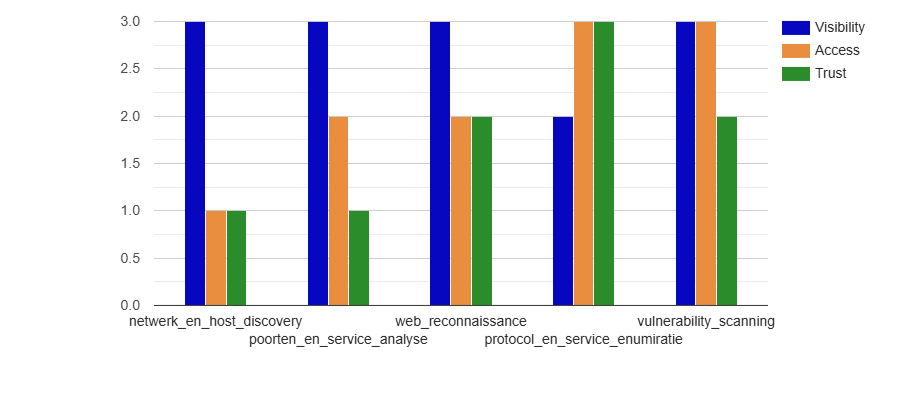
\includegraphics[width=\linewidth]{RAV_vergelijking_manueel_BarChart.png}
\caption{RAV vergelijking per tool van de manuele reconnaissance}
\label{fig:rav_barplot_manueel}
\end{figure}


Deze RAV-scores toont aan dat geen enkele tool over de drie secties uitsteekt.
\textit{Protocol en service enumeratie} geeft de meest gebalanceerde resultaten, met hoge scores voor access en trust, maar een lagere visibility, dit suggereert dat deze sectie zeer gedetailleerd is, maar minder zichtbare informatie kan verzamelen.
\textit{Netwerk en host discovery}, \textit{poorten en service analyse} en \textit{scoren hoog & Web reconnaissance} scoren hoog voor visibility, maar wisselend op access en trust. Dit reflecteert hun focus, het identificeren van hosts, poorten en services.
\textit{Vulnerability scanning} toont hoge scores voor visibility en acces, maar een lagere trust score.
Deze resultaten zijn verkregen door gekende commando's te gebruiken, de uitkomsten te evalueren en op basis hiervan vervolgcommando's te bepalen of op te zoeken.

Dit iteratieve proces verklaart waarom de uitvoeringstijd hier twee tot drie dagen bedraagt.
De tijd voor installatie en troubleshooting (niet-werkende commando's, alternatieven bedenken) wordt niet meegenomen in de uitvoeringstijd.
% Ook moet er gemeld worden dat de tijd dat genoemen werdt om geen valiede comanando's te laten uitvoeren en bedenken hier niet in de uitvoeringstijd is meegerekend.


\section{Automatisatie reconnaissance}

De automatisatie van de reconnaissancefase is uitgevoerd met behulp van zeven verschillende tools.
Deze tools verzamelen verschillende taken als scanning, service enumeratie en vulnerability mapping in een herhaalbare workflow.
Ook al zijn deze tools krachtig, is niet iedere tool geschikt voor een gecontroleerde omgeving zonder toegang tot het internet.
De tools die internet nodig hebben voor OSINT taken uit te voeren, zoals Shodan, Spiderfoot, Amass en Recon-ng, zijn uitgesloten van de volledige analyse, maar worden wel erkend voor de volledigheid.

Iedere tool is individueel en vergelijkend onderzocht, gebaseerd op hun technische gedrag, de output kwaliteit en betrouwbaarheid. Alsook op hun Uitvoeringstijd en de OSSTMM RAV-score.

Enkel de tools die volledig kunnen werken binnen in een lokaal netwerk zijn gebruikt.
Iedere tool werd geconfigureerd om de metasploitable2 te scannen, dit met de standaard of lichtelijke aanpassingen.
Alle data was verzameld voor de vergelijkende studie en een RAV-score.

\subsection{AutoRecon}
AutoRecon is een multi threaded enumeratie tool die een grote variatie heeft aan onderliggende scanning tools als Nmap, Feroxbuster, Nikto en meer.
Het detecteert automatisch open poorten, enumereert gelinkte services en verzameld relevante banners en metadata~\autocite{AutoRecon}. 
AutoRecon was getest in meerdere configuraties, waaronder de single-target en full-port scans 

% Deze tool past de flow van de scan af aan de voorafgaande scans en op basis hiervan verdere stappen ondernemen . 
% Hier integreert AutoRecon tools als Nmap, Feroxbuster, Nikto en meer voor een volledige reconnaissance scan.

\begin{itemize}
  \item \textbf{Sterktes:} hoge aanpasbaarheid, diepe integratie van meerdere tool, gestructureerde rapportering.
  \item \textbf{Limitaties:} relatieve hoge uitvoeringstijd veroorzaakt door de uitgebreide scanning.
  \item \textbf{Uitvoeringstijd:} ~78 minuten.
  \item \textbf{RAV-score:}
    {\small
    \begin{itemize}
      \item \textbf{Visibility:} hoog, haalde succesvol meerdere open poorten en service details. 
      \item \textbf{Access:} medium, capabel om de applicatie laag binnen te gaan en de specifieke service fingerprints te identificeren. 
      \item \textbf{Trust:} laag, geeft merendeel publieke informatie zonder gevoelige credentials en bestanden bloot te leggen. 
    \end{itemize}
    } 
\end{itemize}
\newpage

\subsection{CyberScan}

CyberScan is een snelle en lichte scanner ontworpen om open poorten en services te identificeren. 
De voornaamste rol is de snelle enumeratie om de host-beschikbaarheid en basis services te detecteren \autocite{Cyberscan}.

\begin{itemize}
  \item \textbf{Sterktes:} zeer snel, efficiënt voor een eerste verkenning.
  \item \textbf{Limitaties:} mist diepte in de scans en heeft geen vulnerability detectie.
  \item \textbf{Uitvoeringstijd:} ~5 minuten.
  \item \textbf{RAV-score:}
    \small{
    \begin{itemize}
      \item \textbf{Visibility:} medium, basis poort en protocol detectie.
      \item \textbf{Access:} laag, heeft geen service fingerprinting of vulnerablility scanning gedaan.
      \item \textbf{Trust:} geen, de output bevat geen gevoelige informatie. 
    \end{itemize}
    }
\end{itemize}

\subsection{Sn1per}
Sn1per is een volledig offensieve security scanner dat de reconnaissance aanvult met vulnerablility scanning en rapportage. 
Deze tool presteerde gelijkaardig met AutoRecon, maar geeft ook een gelimiteerde vulnerability analyse zoals standaard credential controles en openstaande admin interfaces \autocite{sn1per}.

\begin{itemize}
  \item \textbf{Sterktes:} rijke features, gecombineerd met meerdere scanning fases in één uitvoer.
  \item \textbf{Limitaties:} hoger systeem verbruik.
  \item \textbf{Uitvoeringstijd:} ~68 minuten.
  \item \textbf{RAV-score:}
    \small{
    \begin{itemize}
      \item \textbf{Visibility:} hoog, gedetailleerde outputs aan poorten, services en http endpoints.
      \item \textbf{Access:} medium, heeft een standaard vulnerability controle.
      \item \textbf{Trust:} medium, sommige zwakke configuraties en standaard instellingen waren blootgelegd.
    \end{itemize}
    }
\end{itemize}


\subsection{RustScan}

RustScan is geoptimaliseerd voor snelle poortscan's. 
Deze tool voert geen service enumeratie uit als standaard, maar kan in samenwerking met Nmap werken \autocite{RustScan}. 

\begin{itemize}
  \item \textbf{Sterktes:} buitengewone performatie, ideaal voor het scannen van grote IP-ranges.
  \item \textbf{Limitaties:} heeft toegevoegde tools nodig voor de volledige functionaliteit. 
  \item \textbf{Uitvoeringstijd:} minder dan 1 minuut.
  \item \textbf{RAV-score:}
    \small{
    \begin{itemize}
      \item \textbf{Visibility:} hoog, deedt een complete poortscan in slechts enkele seconden.
      \item \textbf{Access:} laag, staat niet in contact met services. 
      \item \textbf{Trust:} geen, heeft geen contact met services.
    \end{itemize}
    }
\end{itemize}

\subsection{Nuclei}
Nuclei is een template gebaseerde scanner, gebruikt om problemen zoals open panelen, misconfiguraite en verouderde software componenten te vinden \autocite{Nuclei}.

\begin{itemize}
  \item \textbf{Sterktes:} precisie scanning gebruik makende van community voorbeelden en makkelijk aanpasbaar.
  \item \textbf{Limitaties:} niet geschikt voor standalone gebruik in reconnaissance.
  \item \textbf{Uitvoeringstijd:} ~3 minuten.
  \item \textbf{RAV-score:}
    \small{
    \begin{itemize}
      \item \textbf{Visibility:} laag, afhankelijk van een eerder gekende enumeratie voor input. 
      \item \textbf{Access:} medium, identificeert gekende kwetsbaarheden gebaseerd op de analyse.
      \item \textbf{Trust:} hoog, capabel om verschillende misconfiguraties en gevoelige endpoints weer te geven.
    \end{itemize}
    }
\end{itemize}

\subsection{LazyRecon}
LazyRecon is gemaakt om de reconnaissance makkelijker te maken door tools samen te zetten in een geautomatiseerd script. 
In een internet-gelimiteerde omgeving zijn de OSINT functionaliteiten uitgeschakeld, resulterende in een gelimiteerde capaciteit \autocite{lazyrecon}.

\begin{itemize}
  \item \textbf{Sterktes:} simpele interface, geïntegreerd met meerdere tools.
  \item \textbf{Limitaties:} sterk vertrouwen in online bronnen, de offline functionaliteit is beperkt. 
  \item \textbf{Uitvoeringstijd:} ~9 minuten.
  \item \textbf{RAV-score:}
    \small{
    \begin{itemize}
      \item \textbf{Visibility:} medium, interne scan modules identificeren sommige lokale services en web applicaties.
      \item \textbf{Access:} laag, geen mogelijkheid om meer geavanceerdere scans te doen door de offline status.
      \item \textbf{Trust:} geen, geen gevoelige data gedetecteerd. 
    \end{itemize}
    }
\end{itemize}

\subsection{ReconFTW}

ReconFTW is een geavanceerde automatisatietool gemaakt voor een volledige reconnaissance. Net zoals LazyRecon zijn veel van de de functionaliteiten OSINT gebaseerd. 
In de offline mode geeft het nog steeds bruikbare scans binnenin het interne netwerk \autocite{reconftw}.

\begin{itemize}
  \item \textbf{Sterktes:} groote functionaliteit bij internet-gebaseerde enumeratie.
  \item \textbf{Limitaties:} grote limitatie offline.
  \item \textbf{Uitvoeringstijd:} ~14 minuten.
  \item \textbf{RAV-score:} 
    \small{
    \begin{itemize}
      \item \textbf{Visibility:} medium, onderzoekt toegangbare services en pagina's.
      \item \textbf{Access:} laag, verminderd door een niet internet-gebaseerde enumeratie.
      \item \textbf{Trust:} laag, minimale, gevoelige informatie achterhaald. 
    \end{itemize}
    }
\end{itemize}

\section{Resultatenanalyse geautomatiseerde reconnaissance}

De evaluatie van de tools is gebaseerd op hun betrouwbaarheid, uitvoeringstijd, bruikbaarheid, het CPU-gebruik en de RAV-score. 
In dit deel wordt analyse ondersteund door een staafdiagram die de RAV-scores voor elke tool visualiseert.  

\begin{figure}[H] 
\centering
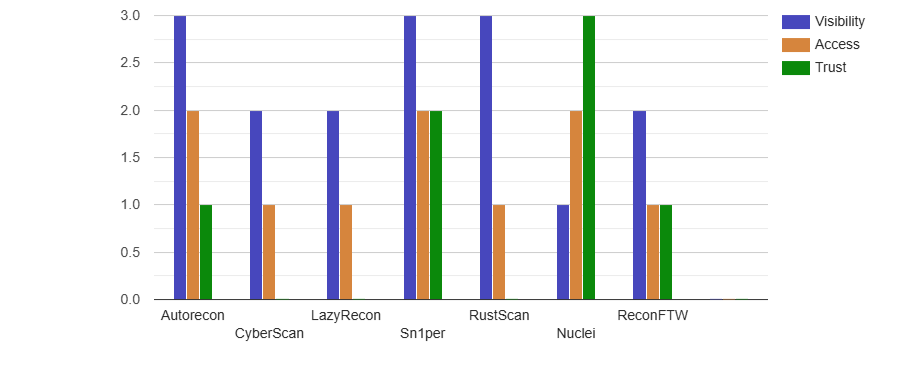
\includegraphics[width=\linewidth]{RAV_vergelijking_geautomatiseerd_BarChart.png}
\caption{RAV vergelijking per tool van de geautomatiseerde reconnaisansse}
\label{fig:rav_barplot_automatisatie}
\end{figure}

Deze RAV-score vergelijking laat zien dat geen enkele tool over al de drie secties uitsteekt. 
AutoRecon en Sn1per geven de meest gebalanceerde resultaten, met een hoge visibility en een gemiddelde access. Deze goede resultaten komen ten koste van een langere uitvoeringstijd.
Rustscan is onovertroffen in snelheid en poort scan's, terwijl Nuclei uitsteekt met zijn vulnerability detectie.
CyberScan en LazyRecon zijn op hun beurt ook geschikt voor snelle scans en ReconFTW, ondanks de offline-modus zijn ze nog steeds in staat bruikbare informatie te geven. 

Uit deze resultaten is af te leiden dat de automatisatie binnen de reconnaissance fase de efficiëntie verbetert. 
Iedere automatisatie tool die in deze vergelijking aan bod is gekomen heeft zijn eigen use case, wat op zijn beurt dan weer speelt met de effectiviteit van de tools.
Voor deze studie, met de focus op de reconnaissance fase en het zoveel mogelijk verzamelen van data, zijn de AutoRecon en Sn1per de meest bruikbare tools door hun uitgebreide analyse.

\section{Vergelijking van manueel en geautomatiseerde reconnaissance}
De manuele en de automatisatie reconnaissance zijn vergeleken op basis van betrouwbaarheid, Uitvoeringstijd, bruikbaarheid en de RAV-score.
\subsection{Betroubaarheid}

\begin{itemize}
  \item \textbf{manuele reconnaissance} de manuele reconnaissance is betrouwbaar voor lichtere commando's, maar is kwetsbaar voor foutmeldingen in complexere commando's. De menselijke interpretatie van de output is essentieel ter volledigheid, maar geeft ook een variabiliteit in de resultaten.
  \item \textbf{automatisatie reconnaissance} 
  \begin{itemize}
    \item \textbf{AutoRecon, Sn1per, LazyRecon, RustScan, } Zeer betrouwbaar (90-95\%), occasionele errors met web scans.
    \item \textbf{CyberScan} Redelijk betrouwbaar (85\%) door veroudering en simpliciteit, niet zo consistent.
    \item \textbf{Nuclei, ReconFTW} Redelijk betrouwbaar (50\%) niet veel mogelijkheden door de offline status.
  \end{itemize}
  \item \textbf{conclusie} De manuele aanpak is beter voor gedetailleerde scans, maar is meer onderhevig aan fouten. De automatisatietools zijn betrouwbaarder, maar kunnen de diepgang van de manuele testen niet vervangen.
\end{itemize}

\subsection{Uitvoeringstijd}

\begin{itemize}
  \item \textbf{Manuele reconnaissance} twee tot drie dagen voor de volledige reconnaissancefase. Als dit uitgevoerd wordt door het bash script kan dit verminderen naar ~30 minuten. Echter vertelt dit niet het hele verhaal van de uitvoeringstijd, het merendeel van de tijd gaat naar het verstaan en interpreteren van de output en deze analyseren voor een vervolgcommando.
  \newpage
  \item \textbf{Automatisatie reconnaissance} 
  \begin{itemize}
    \item \textbf{CyberScan, RustScan} 5-60 seconden
    \item \textbf{Nuclei} 5-20 minuten
    \item \textbf{AutoRecon} 15-30 minuten
    \item \textbf{ReconFTW, LazyRecon} 15-60 minuten
    \item \textbf{Sn1per} 1-120 minuten
  \end{itemize}
  \item \textbf{conclusie} De automatisatie tools zijn aanzienlijk sneller in uitvoeringstijd dan de manuele reconnaissance, echter is dit niet volledig door de tijd die in beslag wordt genomen voor installatie en configuratie van de tools.
\end{itemize}


\subsection{Bruikbaarheid}
\begin{itemize}
  \item \textbf{Manuele reconnaissance} vereist een grote kennis van de tools en de output, dit kan een probleem zijn bij minder ervaren pentesters.
  \item \textbf{Mutomatisatie reconnaissance} 
  \begin{itemize}
    \item \textbf{AutoRecon, LazyRecon, Sn1per, LazyRecon, ReconFTW} gebruiksvriendelijk en eenvoudig te gebruiken, maar de output kan moeilijker verstaanbaar zijn.
    \item \textbf{CyberScan, Nuclei} enkele kennis van de tool vereist.
  \end{itemize}
  \item \textbf{conclusie} De automatisatietools zorgen ervoor dat de barrière voor de nodige kennis van de tools lager is.
\end{itemize}


\subsection{OSSTMM overeenkomst}
\begin{itemize}
  \item \textbf{Standaardiseren} De manuele aanpak is gestructureerd, maar is afhankelijk van de kennis van de pentester. AutoRecon en Sn1per hebben een makkelijke workflow en zijn gestructureerd.
  \item \textbf{Reproduceerbaar} De manuele aanpak is reproduceerbaar in een gecontroleerde omgeving, geautomatisatiseerde tools zorgen voor meer consistentie.
  \item \textbf{Neutraal} Bij de manuele aanpak zijn alle tools open source en daarvoor neutraal, de meeste tools bij de geautomatiseerde aanpak zijn ook open-source maar LazyRecon en reconFTW gebruiken hun eigen gegevens dat kan leiden tot een lichte bias.
  \item \textbf{Meetbare risico} de RAV-scores zorgen voor de meetbare risico's.
\end{itemize}



% \subsection{OSSTMM-Aligned Testing Protocol}

% \begin{itemize}
%   \item \textbf{Pre-Test fase}:
%   \begin{itemize}
%     \item defineer de Rules of Engagement (RoE) voor iedere tool.
%     \item geef securiy best practices aan.
%     \item configureer de testomgeving.
%   \end{itemize}
  
%   \item \textbf{Test Execution}:
%   \begin{itemize}
%     \item test de tool tegen Metasploitable 2.
%     \item documenteer iedere stap van de configuratie. 
%     \item documenteeer de systeem 
%     \item Monitored systeem gegevens (CPU, memory, netwerk)
%   \end{itemize}
  
%   \item \textbf{Post-Test analyse}:
%   \begin{itemize}
%     \item verzamel outputs en logs van de tools.
%     \item analyseer de resultaten.
%     \item berken de RAV score.
%   \end{itemize}
% \end{itemize}

% \section{tool evaluatie}

% \subsection{Network Scanning Suite}

% \subsubsection{Nmap Advanced Features}
% \begin{itemize}
%   \item \textbf{Scripting Engine}:
%   \begin{itemize}
%     \item 600+ NSE scripts categorized by:
%     \begin{itemize}
%       \item Discovery (35\%)
%       \item Vulnerability (25\%)
%       \item Exploit (15\%)
%       \item Miscellaneous (25\%)
%     \end{itemize}
%   \end{itemize}
  
%   \item \textbf{Performance Optimization}:
%   \begin{itemize}
%     \item Timing templates (-T0 to -T5)
%     \item Parallel scan algorithms
%     \item Adaptive host discovery
%   \end{itemize}
% \end{itemize}

% \begin{minted}[linenos,breaklines,frame=single]{bash}
% nmap -sV -sC -p- -T4 \
%      -oA scan_results \
%      target_ip
% \end{minted}





